% Options for packages loaded elsewhere
\PassOptionsToPackage{unicode}{hyperref}
\PassOptionsToPackage{hyphens}{url}
\PassOptionsToPackage{dvipsnames,svgnames*,x11names*}{xcolor}
%
\documentclass[
  12pt,
]{article}
\usepackage{lmodern}
\usepackage{amssymb,amsmath}
\usepackage{ifxetex,ifluatex}
\ifnum 0\ifxetex 1\fi\ifluatex 1\fi=0 % if pdftex
  \usepackage[T1]{fontenc}
  \usepackage[utf8]{inputenc}
  \usepackage{textcomp} % provide euro and other symbols
\else % if luatex or xetex
  \usepackage{unicode-math}
  \defaultfontfeatures{Scale=MatchLowercase}
  \defaultfontfeatures[\rmfamily]{Ligatures=TeX,Scale=1}
  \setmainfont[]{Calibri}
\fi
% Use upquote if available, for straight quotes in verbatim environments
\IfFileExists{upquote.sty}{\usepackage{upquote}}{}
\IfFileExists{microtype.sty}{% use microtype if available
  \usepackage[]{microtype}
  \UseMicrotypeSet[protrusion]{basicmath} % disable protrusion for tt fonts
}{}
\makeatletter
\@ifundefined{KOMAClassName}{% if non-KOMA class
  \IfFileExists{parskip.sty}{%
    \usepackage{parskip}
  }{% else
    \setlength{\parindent}{0pt}
    \setlength{\parskip}{6pt plus 2pt minus 1pt}}
}{% if KOMA class
  \KOMAoptions{parskip=half}}
\makeatother
\usepackage{xcolor}
\IfFileExists{xurl.sty}{\usepackage{xurl}}{} % add URL line breaks if available
\IfFileExists{bookmark.sty}{\usepackage{bookmark}}{\usepackage{hyperref}}
\hypersetup{
  pdftitle={Analyzing the Sentiment Towards Ridesharing Services and Public Transportation in Washington D.C.},
  pdfauthor={Mohammad Al-khasawneh},
  colorlinks=true,
  linkcolor=blue,
  filecolor=Maroon,
  citecolor=Blue,
  urlcolor=Blue,
  pdfcreator={LaTeX via pandoc}}
\urlstyle{same} % disable monospaced font for URLs
\usepackage[margin=1in]{geometry}
\usepackage{color}
\usepackage{fancyvrb}
\newcommand{\VerbBar}{|}
\newcommand{\VERB}{\Verb[commandchars=\\\{\}]}
\DefineVerbatimEnvironment{Highlighting}{Verbatim}{commandchars=\\\{\}}
% Add ',fontsize=\small' for more characters per line
\usepackage{framed}
\definecolor{shadecolor}{RGB}{248,248,248}
\newenvironment{Shaded}{\begin{snugshade}}{\end{snugshade}}
\newcommand{\AlertTok}[1]{\textcolor[rgb]{0.94,0.16,0.16}{#1}}
\newcommand{\AnnotationTok}[1]{\textcolor[rgb]{0.56,0.35,0.01}{\textbf{\textit{#1}}}}
\newcommand{\AttributeTok}[1]{\textcolor[rgb]{0.77,0.63,0.00}{#1}}
\newcommand{\BaseNTok}[1]{\textcolor[rgb]{0.00,0.00,0.81}{#1}}
\newcommand{\BuiltInTok}[1]{#1}
\newcommand{\CharTok}[1]{\textcolor[rgb]{0.31,0.60,0.02}{#1}}
\newcommand{\CommentTok}[1]{\textcolor[rgb]{0.56,0.35,0.01}{\textit{#1}}}
\newcommand{\CommentVarTok}[1]{\textcolor[rgb]{0.56,0.35,0.01}{\textbf{\textit{#1}}}}
\newcommand{\ConstantTok}[1]{\textcolor[rgb]{0.00,0.00,0.00}{#1}}
\newcommand{\ControlFlowTok}[1]{\textcolor[rgb]{0.13,0.29,0.53}{\textbf{#1}}}
\newcommand{\DataTypeTok}[1]{\textcolor[rgb]{0.13,0.29,0.53}{#1}}
\newcommand{\DecValTok}[1]{\textcolor[rgb]{0.00,0.00,0.81}{#1}}
\newcommand{\DocumentationTok}[1]{\textcolor[rgb]{0.56,0.35,0.01}{\textbf{\textit{#1}}}}
\newcommand{\ErrorTok}[1]{\textcolor[rgb]{0.64,0.00,0.00}{\textbf{#1}}}
\newcommand{\ExtensionTok}[1]{#1}
\newcommand{\FloatTok}[1]{\textcolor[rgb]{0.00,0.00,0.81}{#1}}
\newcommand{\FunctionTok}[1]{\textcolor[rgb]{0.00,0.00,0.00}{#1}}
\newcommand{\ImportTok}[1]{#1}
\newcommand{\InformationTok}[1]{\textcolor[rgb]{0.56,0.35,0.01}{\textbf{\textit{#1}}}}
\newcommand{\KeywordTok}[1]{\textcolor[rgb]{0.13,0.29,0.53}{\textbf{#1}}}
\newcommand{\NormalTok}[1]{#1}
\newcommand{\OperatorTok}[1]{\textcolor[rgb]{0.81,0.36,0.00}{\textbf{#1}}}
\newcommand{\OtherTok}[1]{\textcolor[rgb]{0.56,0.35,0.01}{#1}}
\newcommand{\PreprocessorTok}[1]{\textcolor[rgb]{0.56,0.35,0.01}{\textit{#1}}}
\newcommand{\RegionMarkerTok}[1]{#1}
\newcommand{\SpecialCharTok}[1]{\textcolor[rgb]{0.00,0.00,0.00}{#1}}
\newcommand{\SpecialStringTok}[1]{\textcolor[rgb]{0.31,0.60,0.02}{#1}}
\newcommand{\StringTok}[1]{\textcolor[rgb]{0.31,0.60,0.02}{#1}}
\newcommand{\VariableTok}[1]{\textcolor[rgb]{0.00,0.00,0.00}{#1}}
\newcommand{\VerbatimStringTok}[1]{\textcolor[rgb]{0.31,0.60,0.02}{#1}}
\newcommand{\WarningTok}[1]{\textcolor[rgb]{0.56,0.35,0.01}{\textbf{\textit{#1}}}}
\usepackage{graphicx,grffile}
\makeatletter
\def\maxwidth{\ifdim\Gin@nat@width>\linewidth\linewidth\else\Gin@nat@width\fi}
\def\maxheight{\ifdim\Gin@nat@height>\textheight\textheight\else\Gin@nat@height\fi}
\makeatother
% Scale images if necessary, so that they will not overflow the page
% margins by default, and it is still possible to overwrite the defaults
% using explicit options in \includegraphics[width, height, ...]{}
\setkeys{Gin}{width=\maxwidth,height=\maxheight,keepaspectratio}
% Set default figure placement to htbp
\makeatletter
\def\fps@figure{htbp}
\makeatother
\setlength{\emergencystretch}{3em} % prevent overfull lines
\providecommand{\tightlist}{%
  \setlength{\itemsep}{0pt}\setlength{\parskip}{0pt}}
\setcounter{secnumdepth}{-\maxdimen} % remove section numbering
\usepackage{booktabs}
\usepackage{longtable}
\usepackage{array}
\usepackage{multirow}
\usepackage{wrapfig}
\usepackage{float}
\usepackage{colortbl}
\usepackage{pdflscape}
\usepackage{tabu}
\usepackage{threeparttable}
\usepackage{threeparttablex}
\usepackage[normalem]{ulem}
\usepackage{makecell}
\usepackage{xcolor}

\title{Analyzing the Sentiment Towards Ridesharing Services and Public
Transportation in Washington D.C.}
\usepackage{etoolbox}
\makeatletter
\providecommand{\subtitle}[1]{% add subtitle to \maketitle
  \apptocmd{\@title}{\par {\large #1 \par}}{}{}
}
\makeatother
\subtitle{GitHub: \url{https://github.com/mbmk2020/FOCD2021_Final_Project}}
\author{Mohammad Al-khasawneh}
\date{2021-12-13}

\begin{document}
\maketitle

{
\hypersetup{linkcolor=}
\setcounter{tocdepth}{2}
\tableofcontents
}
\newpage

\hypertarget{introduction}{%
\section{Introduction}\label{introduction}}

The growth of the population and their mobility needs require other
alternative transportation systems such as ride-sharing services. The
ride-sharing services are more promising for people's needs in terms of
cost and time since they are app-based use smartphone technology in
their functionality. They can be considered a potential solution to meet
the needs of passengers in terms of flexibility and cost without
expanding the service frequency of public transportation. Both of these
ride services are highly demanding in the metropolitan where people tend
to avoid driving or having their cars to avoid delays or parking
difficulties accompanied by the dense population in the area. The first
impression about these ride services is that Public transportation is
usually cheaper than ride-sharing services. On the other hand,
ride-sharing services may be faster and easier to access. The main
objective of this research project is to answer these questions through
a sentiment analysis for people's Twitter posts to extract their
feelings about the available alternatives of public transportation and
ride-sharing services. The Washington D.C. metropolitan area is selected
as the geographical area for this study. Three services included Uber,
Lyft, and the normal Taxi are selected to study people's opinions about
ride-sharing services, whereas the Amtrak, Metro, and Metrobus were
selected to study people's opinions about the public transportation
services. Social media has become more popular and is widely used by
people of all ages. Twitter is one of the most popular social media with
millions of active users monthly. Many organizations, business companies
specifically, use this social media to gain some feedback for their
business.

\hypertarget{motivation}{%
\section{Motivation}\label{motivation}}

The motivation for doing this research project is to answer the
questions of what people prefer to use: public transportation or
ridesharing services through a sentiment analysis using Twitter posts.
Both Twitter data and sentiment analysis are motivated keys for the
project. Several research studies have been done in the field of
transportation engineering using sentiment analysis. Sonia et
al.~(\protect\hyperlink{ref-Sonia16}{2016}) have used Twitter data to
measure and compare customer satisfaction between two companies that
provide online transportation services. They used the sentiment analysis
technique and found that most of the Twitter posts were for bad
experiences with these two companies. Another study by Eddendy et
al.~(\protect\hyperlink{ref-Effendy16}{2016}) conducted sentiment
analysis for Twitter posts about the use of public transportation in the
big cities in Indonesia. These research studies have provided good
examples of how Twitter data and sentiment analysis can be used in the
field of transportation engineering. Therefore, I was motivated to do a
comprehensive comparison to include both the public transportation and
the ridesharing services in one comparison. Another reason that
motivates me to choose twitter data is that people get the chance to
speak more honestly there about their opinions.

\hypertarget{installing-scripts}{%
\section{Installing Scripts}\label{installing-scripts}}

\hypertarget{required-packages}{%
\subsection{Required packages}\label{required-packages}}

The following are the packages used in this research project. The
``twitterR'' package was used for search twitter data with specific
geographical location and search terms. The ``tidytext'' and ``dplyer''
packages were used for data manipulation. Finally, the packages of
``ggmap'' and ``gridExtra'' were used for data visualization and plot
organizations.

\begin{Shaded}
\begin{Highlighting}[]
\KeywordTok{install.packages}\NormalTok{(}\KeywordTok{c}\NormalTok{(}\StringTok{"mnormt"}\NormalTok{, }\StringTok{"psych"}\NormalTok{, }\StringTok{"SnowballC"}\NormalTok{,}
                   \StringTok{"hunspell"}\NormalTok{,}\StringTok{"broom"}\NormalTok{, }\StringTok{"tokenizers"}\NormalTok{, }\StringTok{"janeaustenr"}\NormalTok{))}
\KeywordTok{install.packages}\NormalTok{(}\StringTok{"twitteR"}\NormalTok{)}
\KeywordTok{install.packages}\NormalTok{(}\StringTok{"tidytext"}\NormalTok{)}
\KeywordTok{install.packages}\NormalTok{(}\StringTok{"ggmap"}\NormalTok{)}
\KeywordTok{install.packages}\NormalTok{(}\StringTok{"tcltk"}\NormalTok{)}
\KeywordTok{install.packages}\NormalTok{(}\StringTok{"gridExtra"}\NormalTok{)}
\KeywordTok{install.packages}\NormalTok{(}\StringTok{"dplyr"}\NormalTok{)}
\KeywordTok{install.packages}\NormalTok{(}\StringTok{"kableExtra"}\NormalTok{)}
\KeywordTok{install.packages}\NormalTok{(}\StringTok{"sentimentr"}\NormalTok{)}
\end{Highlighting}
\end{Shaded}

\hypertarget{required-libraries}{%
\subsection{Required libraries}\label{required-libraries}}

The following are the specific libraries used in this project.

\begin{Shaded}
\begin{Highlighting}[]
\KeywordTok{library}\NormalTok{(twitteR)}
\KeywordTok{library}\NormalTok{(tidyverse)}
\KeywordTok{library}\NormalTok{(tidytext)}
\KeywordTok{library}\NormalTok{(ggmap)}
\KeywordTok{library}\NormalTok{(tcltk)}
\KeywordTok{library}\NormalTok{(gridExtra)}
\KeywordTok{library}\NormalTok{(scales)}
\KeywordTok{library}\NormalTok{(dplyr)}
\KeywordTok{library}\NormalTok{(kableExtra)}
\KeywordTok{library}\NormalTok{(sentimentr)}
\end{Highlighting}
\end{Shaded}

\hypertarget{setup-the-twitter-api}{%
\subsection{Setup the twitter API}\label{setup-the-twitter-api}}

In order to be able to use the twitter API the following are the keys
and tokens requested through twitter developer website
\url{https://developer.twitter.com/en} in order to be able to use the
twitter API.

\begin{Shaded}
\begin{Highlighting}[]
\CommentTok{# The keys were hidden for privacy.}

\NormalTok{consumer_key <-}\StringTok{ "consumer_key_XX"}
\NormalTok{consumer_secret <-}\StringTok{ "consumer_secret_XX"}
\NormalTok{access_token <-}\StringTok{ "access_token_XX"}
\NormalTok{access_secret <-}\StringTok{ "access_secret_XX"}

\CommentTok{# This step is needed to setup the twitter API and before we start }
\CommentTok{# searching for data. It made as comment because the keys have to be real }
\CommentTok{# and active in order to run this line without errors. If you set your keys }
\CommentTok{# you can remove the "#" and run this line: }

\CommentTok{# setup_twitter_oauth(consumer_key, consumer_secret, access_token, }
\CommentTok{#                     access_secret)}
\end{Highlighting}
\end{Shaded}

\hypertarget{data}{%
\section{Data}\label{data}}

The first part of the project is data gathering. The data used in this
study was mainly from twitter posts. The data obtained from twitter API
using `twitterR' package. The API provides the user with an access token
that gives the user access to searching for tweets and information about
them and stores them in a data frame. The data includes people twitter
posts about the available public transportation: Amtrak, Metro, and
Metrobus services and also the ridesharing services including: Uber,
Lyft, and the normal cab Taxi. The obtained data covered mainly the area
of Washington D.C. and up to Baltimore area as many of these ride
services lives in Baltimore as well. Since The twitter API gives only
access to the most recent 8 days, the data for this project was combined
for four separate searches conducted on following dates: Nov 2nd, Nov
12, Nov 22, and Dec 2nd.

\hypertarget{searching-data-using-twitter-api}{%
\subsection{Searching data using twitter
API}\label{searching-data-using-twitter-api}}

The following is the code used to search for Twitter posts about each
ride service:

\begin{Shaded}
\begin{Highlighting}[]
\CommentTok{##Ridesharing services}
\CommentTok{#Taxi <- twListToDF(searchTwitter("taxi", geocode = "38.907,-77.036,60mi",}
\CommentTok{#                                  n = 5000,lang="en"))}
\CommentTok{#Uber <- twListToDF(searchTwitter("Uber", geocode = "38.907,-77.036,60mi",}
\CommentTok{#                                  n = 5000,lang="en"))}
\CommentTok{#Lyft <- twListToDF(searchTwitter("Lyft", geocode = "38.907,-77.036,60mi",}
\CommentTok{#                                  n = 5000,lang="en"))}
\CommentTok{#Ridesharing_Services <- rbind(Taxi, Uber, Lyft)}
\CommentTok{##Public transportation}
\CommentTok{#Amtrak <- twListToDF(searchTwitter("amtrak", geocode = "38.907,-77.036,}
\CommentTok{#                                    60mi",n = 5000,lang="en"))}
\CommentTok{#metrobus <- twListToDF(searchTwitter("metrobus", geocode = "38.907,-77.036,}
\CommentTok{#                                      60mi",n = 5000,lang="en"))}
\CommentTok{#metro <- twListToDF(searchTwitter("metro", geocode = "38.907,-77.036,}
\CommentTok{#                                   60mi",n = 5000,lang="en"))}
\CommentTok{#Public_Transportation <- rbind(Amtrak, metro, metrobus)}
\end{Highlighting}
\end{Shaded}

\hypertarget{combining-data-for-one-month-history}{%
\subsection{Combining data for one month
history}\label{combining-data-for-one-month-history}}

The downloaded searches were stored at the local storage and then were
combined into one dataframe for each ride service.

The following table summaries the number of twitter posts obtained for
each ride service:

\begin{tabular}[t]{l|r|r|r|r|r}
\hline
  & 11.02.2021 & 11.12.2021 & 11.22.2021 & 12.02.2021 & Total\\
\hline
Uber & 1712 & 1475 & 1339 & 1322 & 5848\\
\hline
Lyft & 564 & 360 & 335 & 282 & 1541\\
\hline
Taxi & 319 & 444 & 415 & 254 & 1432\\
\hline
Amtrak & 354 & 371 & 363 & 243 & 1331\\
\hline
Metro & 2418 & 1763 & 1687 & 1624 & 7492\\
\hline
Metrobus & 47 & 23 & 25 & 21 & 116\\
\hline
\end{tabular}

\hypertarget{data-analysis}{%
\section{Data Analysis}\label{data-analysis}}

After the required data was gathered and stored in data frames. The data
was cleaned out from the uninformative words through some tokenization
steps. Different functions were created to remove ``stop'' words such as
``and'', ``the'', ``of'', ``or'' as well as twitter specific words such
as ``rt'' etc. The function also splits the tweets into individual words
and removes all hashtags and signs.

After tokenizing and cleaning the data, the tweets were fed to specific
functions of each package. For the first packages ``tidytext'', the
function takes the tweets and returns a score for each tweet. This score
is then classified according to a function coded into positive and
negative and their the score which represent the repetitive of each
word.

Finally, a data table is created from the positive and negative
classification and a graph is created to visualize the results. The
following section will have more detailed description for each step in
the data analysis.

\hypertarget{data-pre-proccessing-and-tokanization}{%
\subsection{Data Pre-proccessing and
Tokanization}\label{data-pre-proccessing-and-tokanization}}

The following code is for data cleaning and tokenizing:

\begin{Shaded}
\begin{Highlighting}[]
\NormalTok{Tokenization_fun <-}\StringTok{ }\ControlFlowTok{function}\NormalTok{(df)\{}
\NormalTok{  df}\OperatorTok{$}\NormalTok{text =}\StringTok{ }\KeywordTok{gsub}\NormalTok{(}\StringTok{"(f|ht)(tp)(s?)(://)(.*)[.|/](.*)"}\NormalTok{, }\StringTok{" "}\NormalTok{, df}\OperatorTok{$}\NormalTok{text)}
  
  \CommentTok{#removing link}
\NormalTok{  df}\OperatorTok{$}\NormalTok{text =}\StringTok{ }\KeywordTok{gsub}\NormalTok{(}\StringTok{"(f|ht)(tp)(s?)(://)(.*)[.|/](.*)"}\NormalTok{, }\StringTok{" "}\NormalTok{, df}\OperatorTok{$}\NormalTok{text)}

  \CommentTok{# removing hashtags}
\NormalTok{  df}\OperatorTok{$}\NormalTok{text =}\StringTok{ }\KeywordTok{gsub}\NormalTok{(}\StringTok{"#}\CharTok{\textbackslash{}\textbackslash{}}\StringTok{w+"}\NormalTok{, }\StringTok{" "}\NormalTok{, df}\OperatorTok{$}\NormalTok{text)}

  \CommentTok{# removing @people}
\NormalTok{  df}\OperatorTok{$}\NormalTok{text =}\StringTok{ }\KeywordTok{gsub}\NormalTok{(}\StringTok{"@}\CharTok{\textbackslash{}\textbackslash{}}\StringTok{w+"}\NormalTok{, }\StringTok{" "}\NormalTok{, df}\OperatorTok{$}\NormalTok{text)}

  \CommentTok{#removing punctuations}
\NormalTok{  df}\OperatorTok{$}\NormalTok{text =}\StringTok{ }\KeywordTok{gsub}\NormalTok{(}\StringTok{"[[:punct:]]"}\NormalTok{, }\StringTok{" "}\NormalTok{, df}\OperatorTok{$}\NormalTok{text)}

  \CommentTok{#removing numbers}
\NormalTok{  df}\OperatorTok{$}\NormalTok{text =}\StringTok{ }\KeywordTok{gsub}\NormalTok{(}\StringTok{"[[:digit:]]"}\NormalTok{, }\StringTok{" "}\NormalTok{, df}\OperatorTok{$}\NormalTok{text)}

  \CommentTok{#removing emojis}
\NormalTok{  df}\OperatorTok{$}\NormalTok{text <-}\StringTok{ }\KeywordTok{str_replace_all}\NormalTok{(df}\OperatorTok{$}\NormalTok{text,}\StringTok{"[^[:graph:]]"}\NormalTok{,}\StringTok{" "}\NormalTok{)}
\NormalTok{  df}\OperatorTok{$}\NormalTok{text <-}\StringTok{ }\KeywordTok{str_replace_all}\NormalTok{(df}\OperatorTok{$}\NormalTok{text,}\StringTok{'https'}\NormalTok{,}\StringTok{" "}\NormalTok{)}
\NormalTok{  df}\OperatorTok{$}\NormalTok{text <-}\StringTok{ }\KeywordTok{str_replace_all}\NormalTok{(df}\OperatorTok{$}\NormalTok{text,}\StringTok{'amp'}\NormalTok{,}\StringTok{" "}\NormalTok{)}

  \CommentTok{#removing spaces}
\NormalTok{  df}\OperatorTok{$}\NormalTok{text =}\StringTok{ }\KeywordTok{gsub}\NormalTok{(}\StringTok{"[ }\CharTok{\textbackslash{}t}\StringTok{]\{2,\}"}\NormalTok{, }\StringTok{" "}\NormalTok{, df}\OperatorTok{$}\NormalTok{text)}
\NormalTok{  df}\OperatorTok{$}\NormalTok{text =}\StringTok{ }\KeywordTok{gsub}\NormalTok{(}\StringTok{"^}\CharTok{\textbackslash{}\textbackslash{}}\StringTok{s+|}\CharTok{\textbackslash{}\textbackslash{}}\StringTok{s+$"}\NormalTok{, }\StringTok{""}\NormalTok{, df}\OperatorTok{$}\NormalTok{text)}
  
  \KeywordTok{return}\NormalTok{(df)}
\NormalTok{\}}

\NormalTok{Taxi.tweets <-}\StringTok{ }\KeywordTok{Tokenization_fun}\NormalTok{(Taxi.tweets)}
\NormalTok{Uber.tweets <-}\StringTok{ }\KeywordTok{Tokenization_fun}\NormalTok{(Uber.tweets)}
\NormalTok{Lyft.tweets <-}\StringTok{ }\KeywordTok{Tokenization_fun}\NormalTok{(Lyft.tweets)}
\NormalTok{RSS.tweets <-}\StringTok{ }\KeywordTok{rbind}\NormalTok{(Taxi.tweets, Uber.tweets, Lyft.tweets)}


\NormalTok{Amtrak.tweets <-}\StringTok{ }\KeywordTok{Tokenization_fun}\NormalTok{(Amtrak.tweets)}
\NormalTok{metro.tweets <-}\StringTok{ }\KeywordTok{Tokenization_fun}\NormalTok{(metro.tweets)}
\NormalTok{metrobus.tweets <-}\StringTok{ }\KeywordTok{Tokenization_fun}\NormalTok{(metrobus.tweets)}
\NormalTok{PT.tweets <-}\StringTok{ }\KeywordTok{rbind}\NormalTok{(Amtrak.tweets, metro.tweets, metrobus.tweets)}
\end{Highlighting}
\end{Shaded}

After data cleaning and tokenizing. The tweets were passed into
unnset\_tokens() function in order to split them into individual words
using:

\begin{Shaded}
\begin{Highlighting}[]
\CommentTok{#Ride Sharing Services}
\NormalTok{Taxi.tweets_stem <-}\StringTok{ }
\StringTok{  }\NormalTok{Taxi.tweets }\OperatorTok\StringTok{ }\KeywordTok{select}\NormalTok{(text)}\OperatorTok\KeywordTok{unnest_tokens}\NormalTok{(word, text) }\OperatorTok\StringTok{ }
\StringTok{  }\KeywordTok{anti_join}\NormalTok{(stop_words)}
\NormalTok{Uber.tweets_stem <-}\StringTok{ }
\StringTok{  }\NormalTok{Uber.tweets }\OperatorTok\StringTok{ }\KeywordTok{select}\NormalTok{(text)}\OperatorTok\KeywordTok{unnest_tokens}\NormalTok{(word, text) }\OperatorTok\StringTok{ }
\StringTok{  }\KeywordTok{anti_join}\NormalTok{(stop_words)}
\NormalTok{Lyft.tweets_stem <-}\StringTok{ }
\StringTok{  }\NormalTok{Lyft.tweets }\OperatorTok\StringTok{ }\KeywordTok{select}\NormalTok{(text)}\OperatorTok\KeywordTok{unnest_tokens}\NormalTok{(word, text) }\OperatorTok\StringTok{ }
\StringTok{  }\KeywordTok{anti_join}\NormalTok{(stop_words)}
\NormalTok{RSS.tweets_stem <-}\StringTok{ }\KeywordTok{rbind}\NormalTok{(Taxi.tweets_stem,Uber.tweets_stem,Lyft.tweets_stem)}

\CommentTok{#Public Transportation}
\NormalTok{Amtrak.tweets_stem <-}\StringTok{ }
\StringTok{  }\NormalTok{Amtrak.tweets }\OperatorTok\StringTok{ }\KeywordTok{select}\NormalTok{(text)}\OperatorTok\KeywordTok{unnest_tokens}\NormalTok{(word, text) }\OperatorTok\StringTok{ }
\StringTok{  }\KeywordTok{anti_join}\NormalTok{(stop_words)}
\NormalTok{metro.tweets_stem <-}\StringTok{ }
\StringTok{  }\NormalTok{metro.tweets }\OperatorTok\StringTok{ }\KeywordTok{select}\NormalTok{(text)}\OperatorTok\KeywordTok{unnest_tokens}\NormalTok{(word, text) }\OperatorTok\StringTok{ }
\StringTok{  }\KeywordTok{anti_join}\NormalTok{(stop_words)}
\NormalTok{metrobus.tweets_stem <-}\StringTok{ }
\StringTok{  }\NormalTok{metrobus.tweets }\OperatorTok\StringTok{ }\KeywordTok{select}\NormalTok{(text)}\OperatorTok\KeywordTok{unnest_tokens}\NormalTok{(word, text) }\OperatorTok\StringTok{ }
\StringTok{  }\KeywordTok{anti_join}\NormalTok{(stop_words)}
\NormalTok{PT.tweets_stem <-}\StringTok{ }\KeywordTok{rbind}\NormalTok{(Amtrak.tweets_stem, metro.tweets_stem, }
\NormalTok{                        metrobus.tweets_stem)}
\end{Highlighting}
\end{Shaded}

In order to check whether the collected searches have included some
relevant words to transportation or not, the most common words in
people's twitter posts about ridesharing services and public
transportation were counted and ploted as shown in Figure 1.
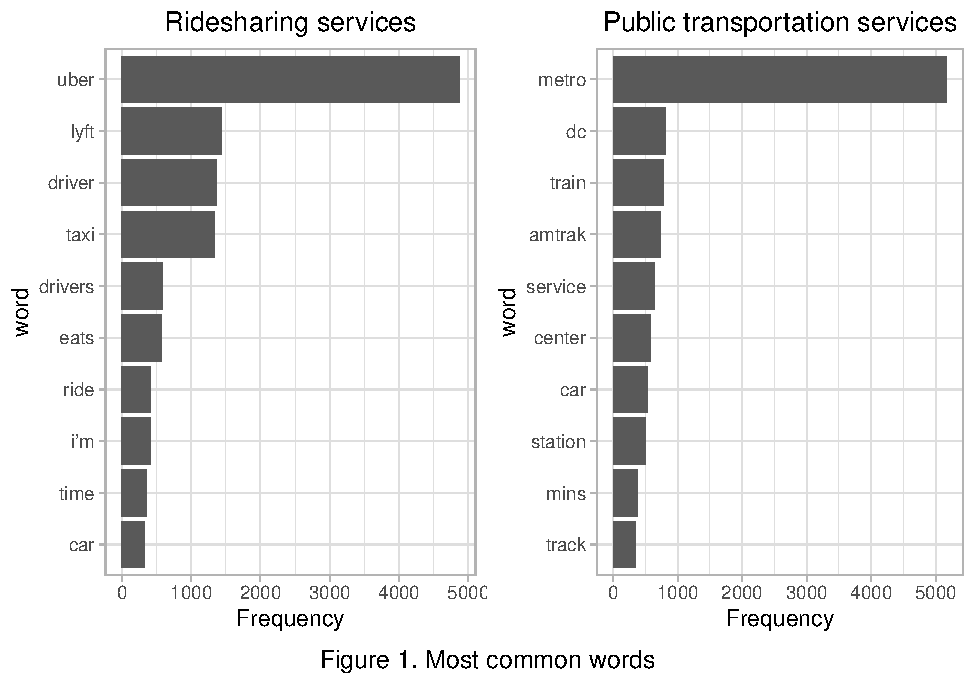
\includegraphics{Class_Project_Report_files/figure-latex/unnamed-chunk-11-1.pdf}

\hypertarget{sentiment-lexicons-using-tidytext}{%
\subsection{Sentiment lexicons using
``tidytext''}\label{sentiment-lexicons-using-tidytext}}

There are several ways for evaluating the opinion or emotion in text.
The sentiment lexicons provides analysis at the word level by splitting
the whole sentence into individual words and then assigns words into
different categories or feelings with specific scores. The sentiment
lexicons can be done using tidytext package in R. There are also several
lexicons such as: bing from (Bing Liu and collaborators, 2004), ncr by
(Saif Mohammad and Peter Turney, 2010) , and AFINN from ( Finn Årup
Nielsen, 2011). The bing sentiment analysis will be used for this
research project for doing the analysis at the word level.

Bing Sentiment Analysis The bing lexicon categorizes words into positive
and negative feelings. The get\_sentiment(``bing'') from
(\protect\hyperlink{ref-tidytext}{2016}) the function was used to obtain
the sentiment dictionary for the list of words prepared by (Bing Liu and
collaborators, 2004). Then the inner\_hoin() was used to match each word
in our data set with the appropriate feelings and sentiment score (-1 or
1). The function sentiment\_score\_bing() was prepared for this project
to to calculate the sentiment score and feeling for each word by by
passing the list of cleaned words from twitter posts. Finally each word
in our dataset about each ride service will were assigned to
``Positive'' or ``Negative'' feelings according to the bing dictionary.
This was done using following code:

\begin{Shaded}
\begin{Highlighting}[]
\NormalTok{sentiment_score_bing <-}\StringTok{ }\ControlFlowTok{function}\NormalTok{(tweets_stem)\{}
\NormalTok{  tweets_stem }\OperatorTok
\StringTok{  }\KeywordTok{inner_join}\NormalTok{(}\KeywordTok{get_sentiments}\NormalTok{(}\StringTok{"bing"}\NormalTok{)) }\OperatorTok
\StringTok{  }\KeywordTok{mutate}\NormalTok{(}\DataTypeTok{value =} \KeywordTok{case_when}\NormalTok{(}
\NormalTok{    sentiment}\OperatorTok{==}\StringTok{"negative"}\OperatorTok{~-}\DecValTok{1}\NormalTok{,}
\NormalTok{    sentiment}\OperatorTok{==}\StringTok{"positive"}\OperatorTok{~}\DecValTok{1}
\NormalTok{  ))}\OperatorTok
\StringTok{  }\KeywordTok{count}\NormalTok{(word, sentiment,value, }\DataTypeTok{sort =} \OtherTok{TRUE}\NormalTok{) }\OperatorTok
\StringTok{  }\KeywordTok{ungroup}\NormalTok{()}
\NormalTok{\}}

\NormalTok{Uber.tweets_Sentiment <-}\StringTok{ }\KeywordTok{sentiment_score_bing}\NormalTok{(Uber.tweets_stem)}
\NormalTok{Lyft.tweets_Sentiment <-}\StringTok{ }\KeywordTok{sentiment_score_bing}\NormalTok{(Lyft.tweets_stem)}
\NormalTok{Taxi.tweets_Sentiment <-}\StringTok{ }\KeywordTok{sentiment_score_bing}\NormalTok{(Taxi.tweets_stem)}
\NormalTok{RSS.tweets_Sentiment <-}\StringTok{ }\KeywordTok{sentiment_score_bing}\NormalTok{(RSS.tweets_stem)}

\NormalTok{Amtrak.tweets_Sentiment <-}\StringTok{ }\KeywordTok{sentiment_score_bing}\NormalTok{(Amtrak.tweets_stem)}
\NormalTok{metro.tweets_Sentiment <-}\StringTok{ }\KeywordTok{sentiment_score_bing}\NormalTok{(metro.tweets_stem)}
\NormalTok{metrobus.tweets_Sentiment <-}\StringTok{ }\KeywordTok{sentiment_score_bing}\NormalTok{(metrobus.tweets_stem)}
\NormalTok{PT.tweets_Sentiment <-}\StringTok{ }\KeywordTok{sentiment_score_bing}\NormalTok{(PT.tweets_stem)}
\end{Highlighting}
\end{Shaded}

The following Figure 2 and Figure 3 show the most common positive and
negative words in the collected twitter posts about the ridesharing
services and the public transportation, respectively.

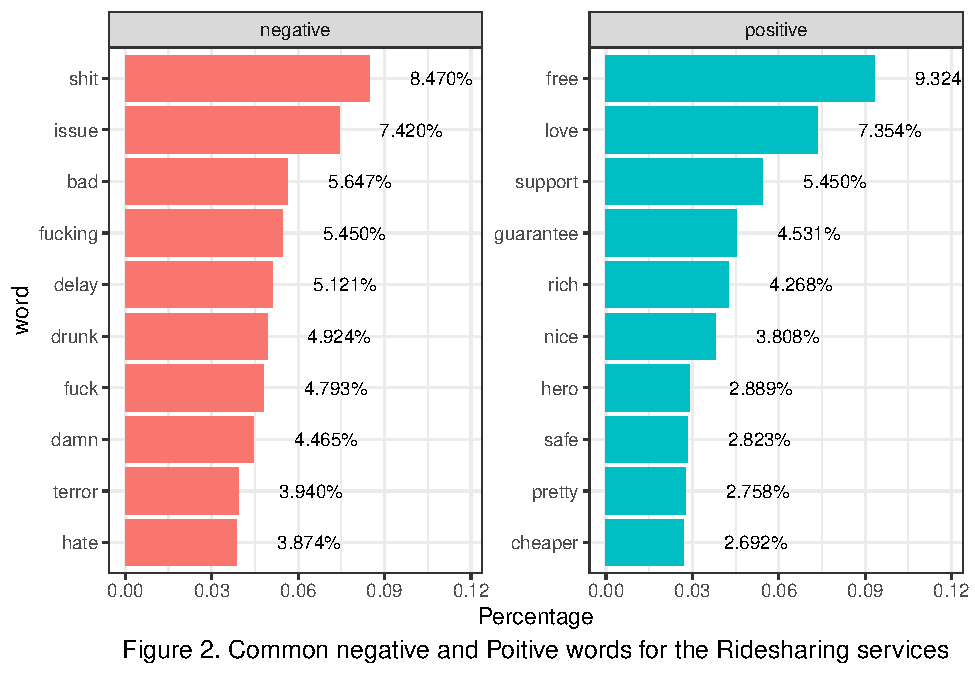
\includegraphics{Class_Project_Report_files/figure-latex/unnamed-chunk-13-1.pdf}
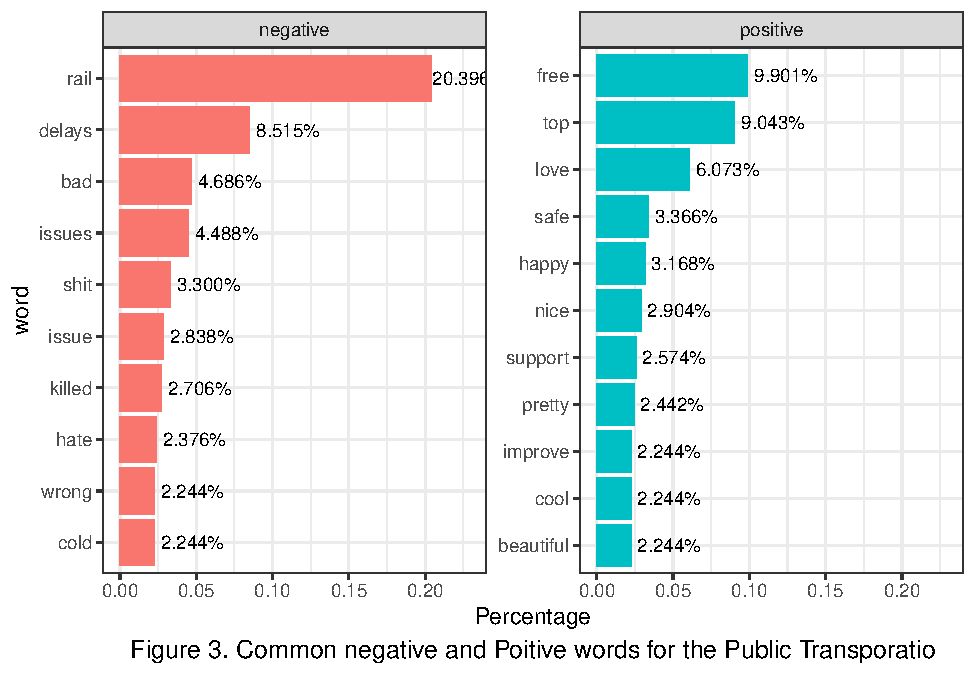
\includegraphics{Class_Project_Report_files/figure-latex/unnamed-chunk-13-2.pdf}

The next step is to count up the positive and negative words for each
ride service. Then the percentage of each category was calculated out of
the total number of words. The following code shows the
total\_sentiment\_score() function used to calculate the percentages of
the positive and negative opinions about the ride service in the
collected twitter posts:

\begin{Shaded}
\begin{Highlighting}[]
\NormalTok{total_sentiment_score <-}\StringTok{ }\ControlFlowTok{function}\NormalTok{(tweets_sentiments, service_name)\{}
\NormalTok{  tweet_table<-tweets_sentiments }\OperatorTok
\StringTok{    }\KeywordTok{mutate}\NormalTok{(}\DataTypeTok{score =}\NormalTok{ n}\OperatorTok{*}\NormalTok{value)}
\NormalTok{  sent.score_positive =}\StringTok{ }\KeywordTok{case_when}\NormalTok{(}
    \KeywordTok{nrow}\NormalTok{(tweet_table)}\OperatorTok{==}\DecValTok{0}\OperatorTok{~}\DecValTok{0}\NormalTok{,}
    \KeywordTok{nrow}\NormalTok{(tweet_table)}\OperatorTok{>}\DecValTok{0}\OperatorTok{~}\KeywordTok{sum}\NormalTok{(tweet_table[tweet_table}\OperatorTok{$}\NormalTok{score}\OperatorTok{>}\DecValTok{0}\NormalTok{,]}\OperatorTok{$}\NormalTok{score)}
\NormalTok{  )}
\NormalTok{  sent.score_negative =}\StringTok{ }\KeywordTok{case_when}\NormalTok{(}
    \KeywordTok{nrow}\NormalTok{(tweet_table)}\OperatorTok{==}\DecValTok{0}\OperatorTok{~}\DecValTok{0}\NormalTok{,}
    \KeywordTok{nrow}\NormalTok{(tweet_table)}\OperatorTok{>}\DecValTok{0}\OperatorTok{~}\KeywordTok{sum}\NormalTok{(tweet_table[tweet_table}\OperatorTok{$}\NormalTok{score}\OperatorTok{<}\DecValTok{0}\NormalTok{,]}\OperatorTok{$}\NormalTok{score)}
\NormalTok{  )}
\NormalTok{  positive_percent =}\StringTok{ }\NormalTok{sent.score_positive}\OperatorTok{/}\NormalTok{(sent.score_positive}\OperatorTok{+}
\StringTok{                                            }\KeywordTok{abs}\NormalTok{(sent.score_negative))}
\NormalTok{  negative_percent =}\StringTok{ }\KeywordTok{abs}\NormalTok{(sent.score_negative)}\OperatorTok{/}\NormalTok{(sent.score_positive}\OperatorTok{+}
\StringTok{                                                 }\KeywordTok{abs}\NormalTok{(sent.score_negative))}
\NormalTok{  results <-}\StringTok{ }\KeywordTok{data.frame}\NormalTok{(}\KeywordTok{c}\NormalTok{(service_name),}\KeywordTok{c}\NormalTok{(}\StringTok{"Positive"}\NormalTok{,}\StringTok{"Negative"}\NormalTok{),}
                        \KeywordTok{c}\NormalTok{(positive_percent,negative_percent))}
  \KeywordTok{colnames}\NormalTok{(results) <-}\StringTok{ }\KeywordTok{c}\NormalTok{(}\StringTok{"Service"}\NormalTok{,}\StringTok{"Sentiment"}\NormalTok{,}\StringTok{"Sentiment_Score"}\NormalTok{)}
  \KeywordTok{return}\NormalTok{(results)}
\NormalTok{\}}
\end{Highlighting}
\end{Shaded}

The sentiment analysis at the word level was performed for each ride
service in order to have individual comparison for each of these
services. Moreover, to have more aggregated comparison, the six services
were reduced to four groups as the following: the Uber and Lyft services
were grouped into one single group of App\_Based Taxi, and the Amtrak
and the Metro were grouped as Train transportation mode. The Figures 4
and 5 illustrate the results from the bing sentiment analysis for the
six different services and the aggregated four groups.

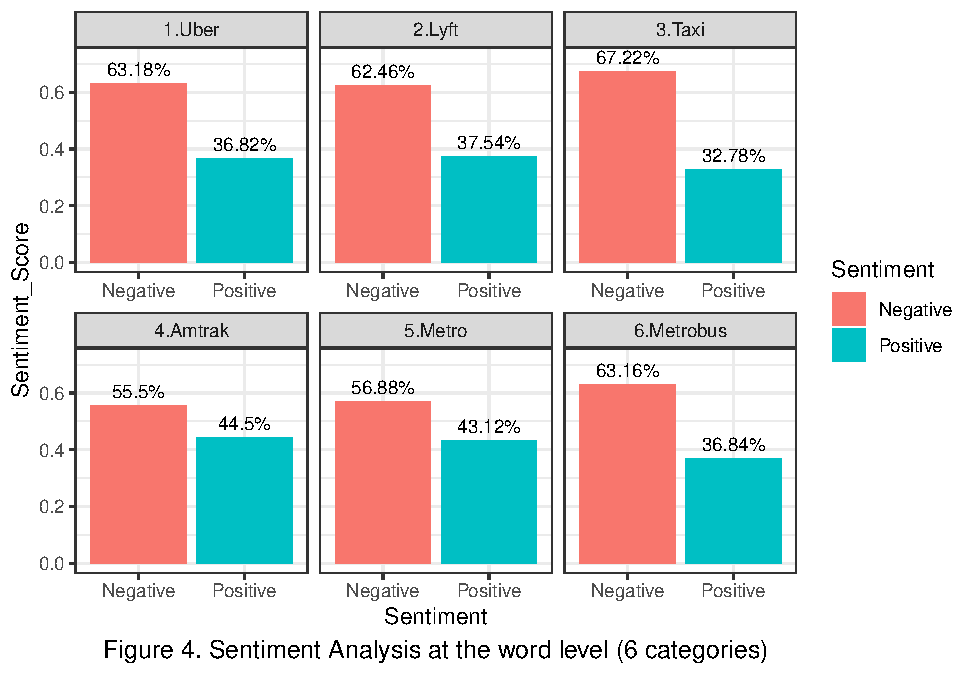
\includegraphics{Class_Project_Report_files/figure-latex/unnamed-chunk-15-1.pdf}

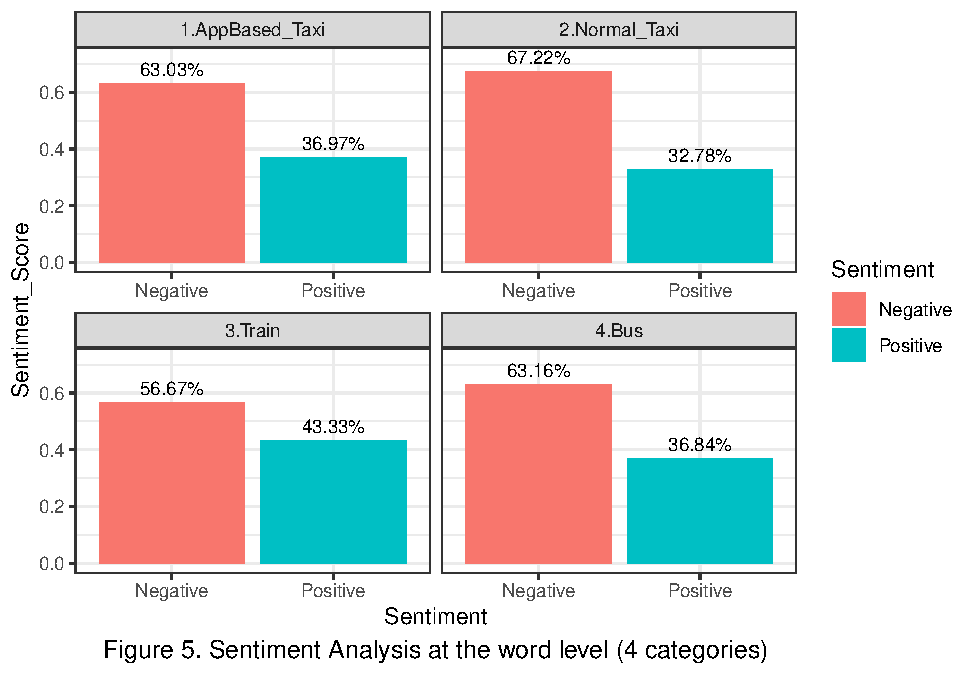
\includegraphics{Class_Project_Report_files/figure-latex/unnamed-chunk-16-1.pdf}

\hypertarget{text-ploarity-analysis-using-sentimentr}{%
\subsection{Text Ploarity Analysis using
sentimentR}\label{text-ploarity-analysis-using-sentimentr}}

For the same six groups and the four groups defined before. The
sentiment analysis was also done at the whole text level using the
(\protect\hyperlink{ref-sentimentr}{2021}) package. The full text or the
twitter post (after cleaning) was considered in the analysis instead of
individual words. This can correct any inversion problem in the text.
For example the bing sentiment would judge ``I do not hate using Uber''
as negative due the ``hate'' word, where in fact it is a positive
opinion.

\begin{Shaded}
\begin{Highlighting}[]
\NormalTok{Text_Polarity_Sentiment <-}\StringTok{ }\ControlFlowTok{function}\NormalTok{(cleaned_data, service_name) \{}
  \KeywordTok{sentiment_by}\NormalTok{(cleaned_data}\OperatorTok{$}\NormalTok{text) }\OperatorTok
\StringTok{  }\KeywordTok{mutate}\NormalTok{(}\DataTypeTok{Sentiment=}\KeywordTok{case_when}\NormalTok{(}
\NormalTok{    ave_sentiment}\OperatorTok{==}\DecValTok{0}\OperatorTok{~}\StringTok{"Natural"}\NormalTok{,}
\NormalTok{    ave_sentiment}\OperatorTok{<}\DecValTok{0}\OperatorTok{~}\StringTok{"Negative"}\NormalTok{,}
\NormalTok{    ave_sentiment}\OperatorTok{>}\DecValTok{0}\OperatorTok{~}\StringTok{"Positive"}
\NormalTok{  )) }\OperatorTok
\StringTok{  }\KeywordTok{select}\NormalTok{(ave_sentiment,Sentiment) }\OperatorTok
\StringTok{  }\KeywordTok{filter}\NormalTok{(Sentiment}\OperatorTok\KeywordTok{c}\NormalTok{(}\StringTok{"Positive"}\NormalTok{,}\StringTok{"Negative"}\NormalTok{)) }\OperatorTok
\StringTok{  }\KeywordTok{group_by}\NormalTok{(Sentiment) }\OperatorTok
\StringTok{  }\KeywordTok{summarise}\NormalTok{(}\DataTypeTok{totals =} \KeywordTok{sum}\NormalTok{(ave_sentiment), }\DataTypeTok{count =} \KeywordTok{n}\NormalTok{())}\OperatorTok
\StringTok{  }\KeywordTok{mutate}\NormalTok{(}\DataTypeTok{Sentiment_Score =}\NormalTok{ count}\OperatorTok{/}\KeywordTok{sum}\NormalTok{(count)) }\OperatorTok
\StringTok{  }\KeywordTok{select}\NormalTok{(Sentiment_Score, Sentiment) }\OperatorTok
\StringTok{  }\KeywordTok{mutate}\NormalTok{(}\DataTypeTok{Service =}\NormalTok{ service_name)}
\NormalTok{\}}
\end{Highlighting}
\end{Shaded}

The Figures 6 and 7 show the results from the sentiment analysis at the
text level using sentimentr package for the six different services and
the aggregated four groups.

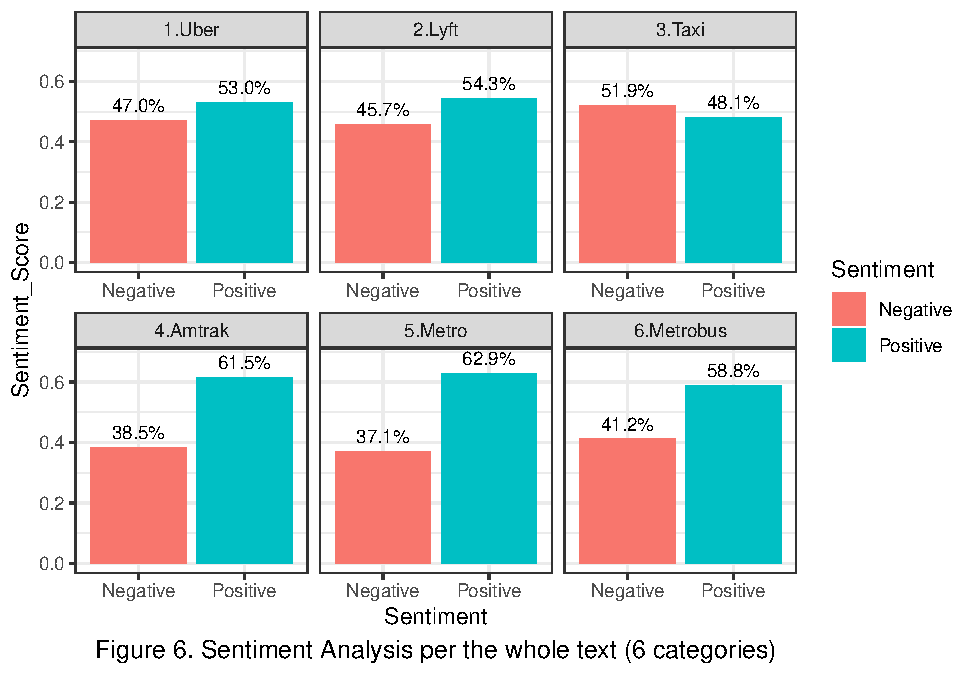
\includegraphics{Class_Project_Report_files/figure-latex/unnamed-chunk-18-1.pdf}

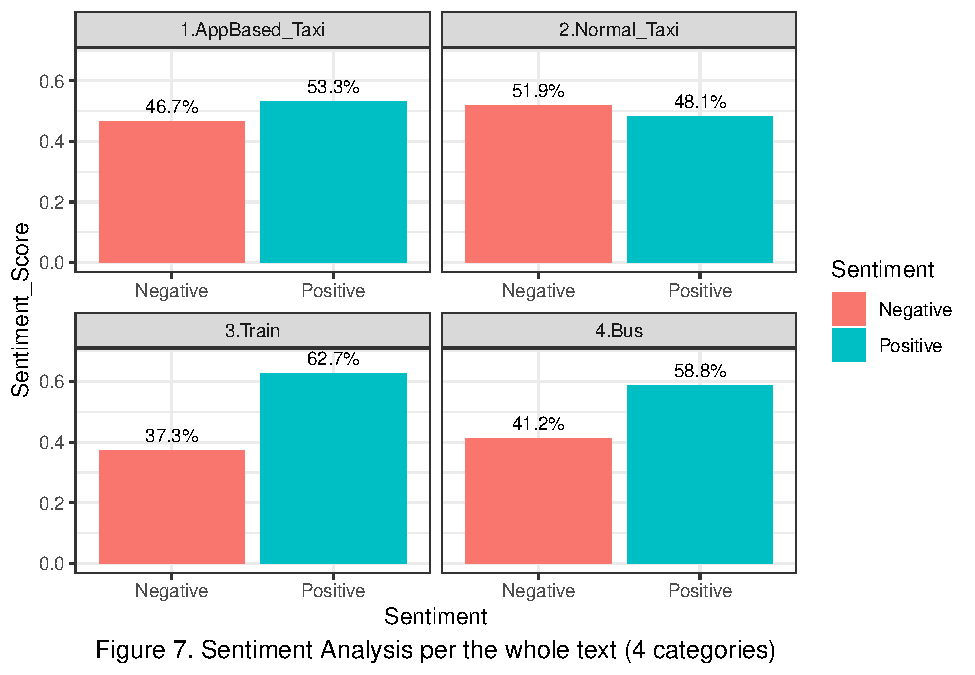
\includegraphics{Class_Project_Report_files/figure-latex/unnamed-chunk-19-1.pdf}

\hypertarget{results}{%
\section{Results}\label{results}}

In general, the sentiment analysis at the word level (Figures 4 and 5)
did not show any strong opinion towrd any of the feelings (positive or
negative) and had slightly differences in the percentages among the
different services. However, the results showed that the App based
services (Uber \& Lyft) had more positive opinions than the normal cab
taxi. Similarly, the Metro and Amtrak results had higher percentages of
the positive feelings than the Metrobus. Moreoever, the results showed
more negative opinions toward the provided services with no significant
differences in the percentages among all the services.

On the other hand, the sentiment analysis at the word level showed that
the twitter posts had more likely positive opinions toward these ride
services expect for the normal cab taxi as shown in Figures 6. Overall,
the relative comparisons between the services was noticed to be the same
or very close between the two method of the sentiment analysis. For
example, the normal cab taxi was always accompanied with the highest
negative opinions and the lowest positive opinions. Therefore, the
services were ranked from the most likely service to the lowest based on
the positive percentages results from both methods. It was found that
both of the two methods had captured very similar ranks for the selected
services. Figures 8 and 9 summaries the ranks for each service or a
group of service for each sentiment analysis method.
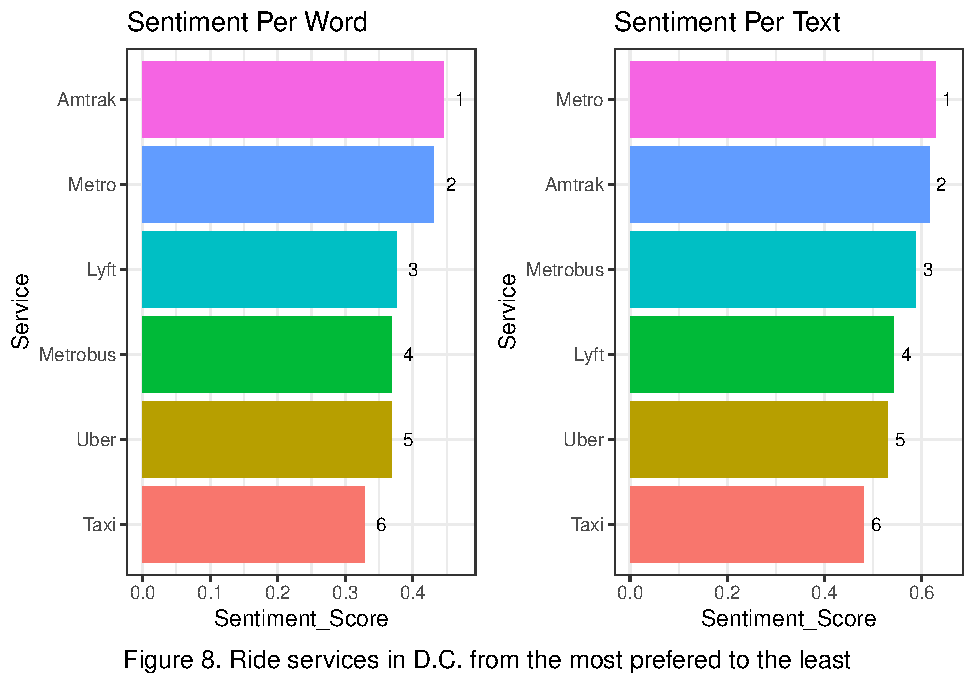
\includegraphics{Class_Project_Report_files/figure-latex/unnamed-chunk-20-1.pdf}

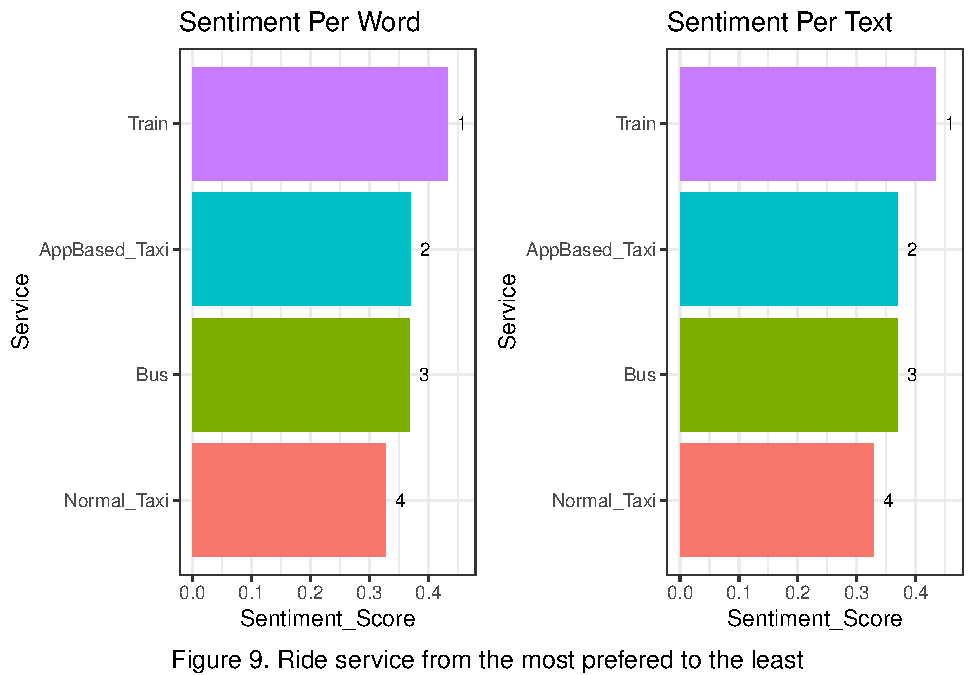
\includegraphics{Class_Project_Report_files/figure-latex/unnamed-chunk-21-1.pdf}

\hypertarget{conclusion}{%
\section{Conclusion}\label{conclusion}}

This research study involves sentiment analysis towards the use of
public transportation and ride-sharing services in the Washington D.C
area. The data was collected through Twitter API for November 2021
(11-02-2021 to 12-02-2021). The collected data included the entire D.C.
area and some parts of Baltimore since several people live there and
work in D.C. The study included several public transportations such as
Amtrak, Metrobus, and the Metro and some common ridesharing services
including Uber, Lyft, and the normal cab-taxi. The sentiment analysis
was done at the word level using the ``tidytext'' package and per the
whole text using the ``bing'' dictionary. The results showed that both
of the methods can be used to measure the same relative comparison
between the service. However, the two methods had opposite opinions
about each service.

\newpage

\hypertarget{references}{%
\section*{References}\label{references}}
\addcontentsline{toc}{section}{References}

\hypertarget{refs}{}
\leavevmode\hypertarget{ref-sentimentr}{}%
Rinker, Tyler W. 2021. \emph{sentimentr: Calculate Text Polarity
Sentiment}. Buffalo, New York.
\url{https://github.com/trinker/sentimentr}.

\leavevmode\hypertarget{ref-tidytext}{}%
Silge, Julia, and David Robinson. 2016. ``Tidytext: Text Mining and
Analysis Using Tidy Data Principles in R.'' \emph{JOSS} 1 (3).
\url{https://doi.org/10.21105/joss.00037}.

\leavevmode\hypertarget{ref-Sonia16}{}%
Sonia Anastasia, Indra Budi. 2016. ``Twitter Sentiment Analysis of
Online Transportation Service Providers.'' Journal Article.
\url{https://ieeexplore.ieee.org/abstract/document/7872807}.

\leavevmode\hypertarget{ref-Effendy16}{}%
Veronikha Effendy, Mira Kania Sabariah, Anita Novantirani. 2016.
``Sentiment Analysis on Twitter About the Use of City Public
Transportation Using Support Vector Machine Method.'' Journal Article.
\url{https://socj.telkomuniversity.ac.id/ojs/index.php/ijoict/article/view/85}.

\end{document}
